\documentclass[10pt,a4paper]{article}
\usepackage[utf8]{inputenc}

% Define the page margin
\usepackage[margin=3cm]{geometry}

% Better typography (font rendering)
\usepackage{microtype}

% Math environments and macros
\usepackage{amsmath}
\usepackage{amsfonts}
\usepackage{amssymb}
\usepackage{amsthm}

% Define \includegraphics to include graphics
\usepackage{graphicx}

% Draw graphics from a text description
\usepackage{tikz}

% Syntax highlighting
\usepackage{minted}

% Set global minted options
\setminted{linenos, autogobble, frame=lines, framesep=2mm}

% Import the comment environment for orgtbl-mode
\usepackage{comment}

% Do not indent paragraphs
\usepackage{parskip}

\title{Network Coding, Sheet 7}
\author{Marten Lienen (03670270)}

\begin{document}

\maketitle

\section*{Exercise 1}

\begin{figure}[h]
  \centering
  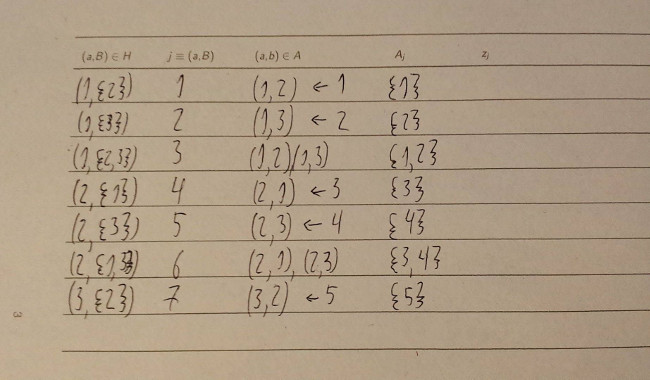
\includegraphics[width=\textwidth]{sheet-7/table}
  \caption{Parts a, b, c, e}
  \label{fig:table}
\end{figure}

\subsection*{Part a)}

See figure \ref{fig:table}.

\subsection*{Part b)}

See figure \ref{fig:table}.

\subsection*{Part c)}

See figure \ref{fig:table}.

\subsection*{Part d)}

See figure \label{fig:part-d}.

\begin{figure}[h]
  \centering
  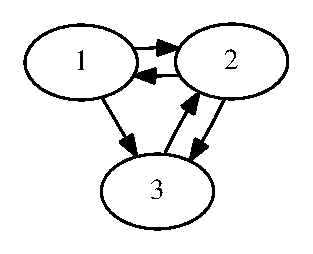
\includegraphics[width=0.3\textwidth]{sheet-7/exercise-1-d}
  \caption{Induced graph}
  \label{fig:part-d}
\end{figure}

\subsection*{Part e)}

See figure \ref{fig:table}.

\subsection*{Part f)}

\begin{equation*}
  N = \begin{pmatrix}
    1 & 0 & 0 & 0 & 0\\
    0 & 1 & 0 & 0 & 0\\
    1 & 1 & 0 & 0 & 0\\
    0 & 0 & 1 & 0 & 0\\
    0 & 0 & 0 & 1 & 0\\
    0 & 0 & 1 & 1 & 0\\
    0 & 0 & 0 & 0 & 1
  \end{pmatrix}
\end{equation*}

\subsection*{Part g)}

\begin{equation*}
  M = \begin{pmatrix}
    1 & 1 & -1 & 0 & 0\\
    -1 & 0 & 1 & 1 & -1\\
    0 & -1 & 0 & -1 & 1
  \end{pmatrix}
\end{equation*}

\subsection*{Part h)}

\begin{equation*}
  Q = \begin{pmatrix}
    1 & 0 & 1 & 0 & 0 & 0 & 0\\
    0 & 1 & 1 & 0 & 0 & 0 & 0\\
    1 & 1 & 1 & 0 & 0 & 0 & 0\\
    0 & 0 & 0 & 1 & 0 & 1 & 0\\
    0 & 0 & 0 & 0 & 1 & 1 & 0\\
    0 & 0 & 0 & 1 & 1 & 1 & 0\\
    0 & 0 & 0 & 0 & 0 & 0 & 1
  \end{pmatrix}
\end{equation*}

\subsection*{Part i)}

\begin{equation*}
  \mathcal{Z} = \bigcup_{\substack{\tau \ge 0\\1^{T}\tau \le 1}} \left\{
    \begin{bmatrix}
      \tau_{1} (1 - \epsilon_{1}) \epsilon_{2}\\
      \tau_{1} (1 - \epsilon_{2}) \epsilon_{1}\\
      \tau_{1} (1 - \epsilon_{1}) (1 - \epsilon_{2})\\
      \tau_{2} (1 - \epsilon_{3}) \epsilon_{4}\\
      \tau_{2} (1 - \epsilon_{4}) \epsilon_{3}\\
      \tau_{2} (1 - \epsilon_{3}) (1 - \epsilon_{4})\\
      \tau_{3} (1 - \epsilon_{5})
    \end{bmatrix}
  \right\}
\end{equation*}

\subsection*{Part j)}

\begin{equation*}
  y = Qz = \begin{pmatrix}
    1 & 0 & 1 & 0 & 0 & 0 & 0\\
    0 & 1 & 1 & 0 & 0 & 0 & 0\\
    1 & 1 & 1 & 0 & 0 & 0 & 0\\
    0 & 0 & 0 & 1 & 0 & 1 & 0\\
    0 & 0 & 0 & 0 & 1 & 1 & 0\\
    0 & 0 & 0 & 1 & 1 & 1 & 0\\
    0 & 0 & 0 & 0 & 0 & 0 & 1
  \end{pmatrix}
  \begin{bmatrix}
    \tau_{1} (1 - \epsilon_{1}) \epsilon_{2}\\
    \tau_{1} (1 - \epsilon_{2}) \epsilon_{1}\\
    \tau_{1} (1 - \epsilon_{1}) (1 - \epsilon_{2})\\
    \tau_{2} (1 - \epsilon_{3}) \epsilon_{4}\\
    \tau_{2} (1 - \epsilon_{4}) \epsilon_{3}\\
    \tau_{2} (1 - \epsilon_{3}) (1 - \epsilon_{4})\\
    \tau_{3} (1 - \epsilon_{5})
  \end{bmatrix} =
  \begin{pmatrix}
    \tau_{1} (1 - \epsilon_{1})\\
    \tau_{1} (1 - \epsilon_{2})\\
    \tau_{1} (1 - \epsilon_{1} \epsilon_{2})\\
    \tau_{2} (1 - \epsilon_{3})\\
    \tau_{2} (1 - \epsilon_{4})\\
    \tau_{2} (1 - \epsilon_{3} \epsilon_{4})\\
    \tau_{3} (1 - \epsilon_{5})
  \end{pmatrix}
\end{equation*}

\subsection*{Part k)}

\begin{equation*}
  Nx = \begin{pmatrix}
    1 & 0 & 0 & 0 & 0\\
    0 & 1 & 0 & 0 & 0\\
    1 & 1 & 0 & 0 & 0\\
    0 & 0 & 1 & 0 & 0\\
    0 & 0 & 0 & 1 & 0\\
    0 & 0 & 1 & 1 & 0\\
    0 & 0 & 0 & 0 & 1
  \end{pmatrix}
  \begin{pmatrix}
    x_{1}\\
    x_{2}\\
    x_{3}\\
    x_{4}\\
    x_{5}
  \end{pmatrix} \le \begin{pmatrix}
    \tau_{1} (1 - \epsilon_{1})\\
    \tau_{1} (1 - \epsilon_{2})\\
    \tau_{1} (1 - \epsilon_{1} \epsilon_{2})\\
    \tau_{2} (1 - \epsilon_{3})\\
    \tau_{2} (1 - \epsilon_{4})\\
    \tau_{2} (1 - \epsilon_{3} \epsilon_{4})\\
    \tau_{3} (1 - \epsilon_{5})
  \end{pmatrix} = y
\end{equation*}

\subsection*{Part l)}

\begin{tabular}{c|c}
  Cut & Value\\
  \hline
  $\{ 1, 2 \}, \{ 3 \}$ & $y_{2} + y_{5} = \tau_{1} (1 - \epsilon_{2}) + \tau_{2} (1 - \epsilon_{4})$\\
  $\{ 1 \}, \{ 2, 3 \}$ & $y_{3} = \tau_{1} (1 - \epsilon_{1} \epsilon_{2})$
\end{tabular}

\subsection*{Part m)}

The minimum of the two cut values.
\begin{equation*}
  r = \min \{ \tau_{1} (1 - \epsilon_{2}) + \tau_{2} (1 - \epsilon_{4}), \tau_{1} (1 - \epsilon_{1} \epsilon_{2}) \}
\end{equation*}

\subsection*{Part n)}

\subsection*{Part o)}

The cut has to be $\{ 1, 3 \}, \{ 2 \}$ and its value is
\begin{equation*}
  y_{1} + y_{7} = \tau_{1} (1 - \epsilon_{1}) + \tau_{3} (1 - \epsilon_{5})
\end{equation*}

\subsection*{Part p)}

\begin{equation*}
  \max_{\substack{\tau \ge 0\\1^{T}\tau = 1}} \min \{ v(S_{1}), v(S_{2}), v(S_{3}) \}
\end{equation*}

\subsection*{Part q)}

\end{document}
